%!TEX root = ../thesis.tex
% ******************************* Thesis Appendix A ****************************
\chapter{Spherical Harmonics on Hyperspheres} 
\label{appendix:spherical-harmonics}

Spherical harmonics are a special set of functions defined on the hypersphere and play a central role in harmonic analysis and approximation theory \citep{wendland2005}. They originate from solving Laplace's equation, and form a complete set of orthogonal functions. Any sufficiently regular function defined on the sphere can be written as a sum of these spherical harmonics, similar to the Fourier series with sines and cosines. Spherical harmonics are defined in arbitrary dimensions \citep{frye2014,dai2013}, but lack explicit formulations and practical implementations in dimensions larger than three. %This is mainly due to the complexity of solving Laplace's equation in higher dimensions.

In this section, we propose a novel algorithm to construct spherical harmonics in $d$ dimensions. The algorithm is based on the existence of a fundamental system of points on the hypersphere, which we select in a greedy fashion through optimisation. This result in spherical harmonics that are a linear combination of zonal functions and form an orthnormal basis on $\dsphere$. The algorithm lends itself well for implementation in Python and TensorFlow, which we provide at: \url{https://github.com/vdutor/SphericalHarmonics}. The code is accompagnied by a series of tests that show that the properties of spherical harmonics, as detailed below, hold. Before outlining the algorithm, we briefly define and cover the important properties of spherical harmonics in $\Reals^d$. We refer the interested reader to \citet{dai2013,frye2014} for a comprehensive overview.
% exist bases of spherical harmonics consisting of entirely zonal harmonics

We adopt the usual $L_2$ inner product for functions $f: \dsphere \rightarrow \Reals$ and $g: \dsphere \rightarrow \Reals$ restricted to the sphere 
\begin{equation}
     \langle f, g\rangle_{L_{2}(\dsphere)} = \frac{1}{\darea} \int_{\dsphere} f(x)\,g(x) \, \calcd{\omega},
\end{equation}
where $\calcd{\omega(x)}$ is the surface area measure such that $\darea$ denotes the surface area of $\dsphere$ 
\begin{equation}
\label{eq:surface}
    \darea = \int_{\dsphere} \calcd{\omega(x)} = \frac{2 \pi ^ {d/2}}{\Gamma(d/2)}.
\end{equation}

Throughout this section we use the following notation and definitions. For $x = (x_1, \ldots, x_d) \in \Reals^d$ and $\alpha = (\alpha_1, \ldots, \alpha_d) \in \Naturals^d$, a monomial $x^\alpha$ is a product $x^\alpha = x_1^{\alpha_1} \ldots x_d^{\alpha_d}$, which has degree $|\alpha| = \alpha_1 + \ldots \alpha_d$. A real homogeneous polynomial $P(x)$ of degree $n$ is a linear combination of monomials of degree $n$ with real coefficients, that is $P(x) = \sum_{|\alpha| = n} c_{\alpha} x^{\alpha}$, with $c_\alpha \in \Reals$. We denote $\mathcal{P}_n^d$ as the space of real homogeneous polynomials of degree $n$, and can show that, counting the cardinality of the set $\{\alpha \in \Naturals^d: |\alpha| = n\}$, that $\dim(\mathcal{P}_n^d) = \binom{n + d -1}{n}$. A function $f:\Reals^d \rightarrow \Reals$ is said to be \emph{harmonic} if $\Delta f = 0$, where $\Delta = \partial_{x_1}^2 + \ldots + \partial_{x_d}^2$ and $\partial_{x_i}$ the partial derivate w.r.t. the $i$-th variable.

\begin{definition}
    The spherical harmonics of degree $n$ of $d$ variables, denoted by $\mathcal{H}_{n}^d$, is the linear space of harmonic and homogeneous in degree $n$ polynomials on $\dsphere$, that is 
    \begin{equation}
        \mathcal{H}_{n}^d = \{p \in \mathcal{P}_n^d: \Delta p = 0\ \text{and}\ p: \dsphere \rightarrow \Reals \}.
    \end{equation}
The dimensionality of $ \mathcal{H}_{n}^d$ is given by
\begin{equation}
\label{eq:numharmonics}
\dim(\mathcal{H}_{n}^d) = \frac{2 n + d - 2}{n} \binom{n + d - 3}{d - 1} := \dnumharmonicsforlevel.
\end{equation}
\end{definition}

The space $\mathcal{H}_{n}^d$ has an orthonormal basis consisting of $\dnumharmonicsforlevel$ functions, denoted by $\{\phi_{n,j}\}_{j=1}^{\dnumharmonicsforlevel}$. The basis satisfy the following properties
\begin{equation}
    \mathcal{H}_{n}^d  = \textrm{span}\left(\phi_{n,1}, \ldots, \phi_{n, \dnumharmonicsforlevel}\right),\quad\text{and}\quad\left\langle \phi_{n, j}, \phi_{n', j'}\right\rangle_{L_2(\dsphere)} = \delta_{n n'} \delta_{j j'}.
\end{equation}

From the completeness and orthonormality of the spherical harmonic basis $\{\phi_{n,j}\}_{n=0,j=1}^{\infty,\dnumharmonicsforlevel}$, it can be shown that they also form a basis of square-integrable functions \citep{frye2014}. This means that we can decompose a function $f: \dsphere \rightarrow \Reals$ as
\begin{equation}
    f = \sum_{n=0}^{\infty} \sum_{j=1}^{\dnumharmonicsforlevel} \widehat{f}_{n, j} \phi_{n, j},\quad\text{with}\quad\widehat{f}_{n, j} = \langle f, \phi_{n, j} \rangle_{L_2(\dsphere)},
\end{equation}
which can be seen as the spherical analogue of the Fourier decomposition of periodic functions onto a basis of sines and cosines.

Subsequently, we will coin the set $\{\phi_{n,j}\}$ as the spherical harmonics. They are indexed by $n$ and $j$, where $n=0,1,2,\ldots$ denotes the degree (or level) and $j=1,\cdots,\dnumharmonicsforlevel$ denotes the orientation of the spherical harmonic. We are interested in finding $\{\phi_{n,j}\}$ in arbitrary dimension. For $d=2$, is solving Laplace's equation ($\Delta p = 0$) directly relatively straightforward. Doing so reveals that $N^{2}_0 = 1$ with $\phi_{0, 1} = 1$ and $N^{2}_n = 2$ for all $n > 0$ with $\phi_{n, 1}(\theta) = \sqrt{2} \cos(n \theta)$ and $\phi_{n, 2}(\theta) = \sqrt{2} \sin(n \theta)$. This shows that on the unit circle $\sphere^1$, the spherical harmonics correspond to the Fourier basis. For $d=3$, we can also directly solve Laplace's diffential equation to find $\dnumharmonicsforlevel = 2n + 1$ and a closed form solution for $\{\phi_{n,j}\}$. However, for $d > 3$, explicit formulations for the spherical harmonics become very rare. To the best of our knowledge, the only explicit formulation we could find is in \citet[Theorem~5.1]{dai2013}, which consists of a product over polynomials. This makes the implementation cumbersome and numerically unstable, and only practically useful up to 10 dimensions \citep{Dutordoir2020spherical}. However, making use of the following two theorems, we can derive another formulation for the basis of spherical harmonics as a sum of polynomials, rather than a product. The connection between spherical harmonics and orthogonal polynomials becomes clear in the next theorem.
\begin{theorem}[Addition]
    \label{theorem:addition}
    Let $\{\phi_{n,j}\}_{j=1}^{\dnumharmonicsforlevel}$ be an orthonormal basis for the spherical harmonics of degree $n$ and $x,x' \in \dsphere$. Then the Gegenbauer polynomial $C_n^{(\alpha)}: [-1, 1] \rightarrow \Reals$ of degree $n$ can be written as
\begin{equation}
    \sum_{j=1}^{\dnumharmonicsforlevel} \phi_{n, j}(x) \phi _{n, j}(x') = \frac{n + \alpha}{\alpha}\,
    C_n^{(\alpha)}(x\transpose x')\quad\text{with}\quad \alpha = \frac{d-2}{2}.
\end{equation}
\end{theorem}
As a result of the relation between the Gegenbauer polynomial and the spherical harmonics, are the Gegenbauer polynomial sometimes referred to as ultraspherical polynomials. For $d=2$, Theorem~1 recovers the addition formula of the cosine function, as indeed $\cos(\theta) \cos(\theta') + \sin(\theta) \sin(\theta') = \cos(\theta - \theta')$ and $C_n^{(0)}(t) = \cos(n \arccos(t))$. The Gegenbauer polynomials with $\alpha=0$ are better known as the Chebyshev polynomials. Another connection between spherical harmonics and Gegenbauer polynomials is given by the Funk-Hecke theorem and applies to zonal functions. A zonal function on $\dsphere$ is a function that is rotationally invariant w.r.t. to a point on the sphere, $\eta \in \dsphere$. This means that the function only depends on the inner product $\eta\transpose x$, or equivalently, on the geodestic distance between $\eta$ and $x$.

\begin{theorem}[Funk-Hecke]
    \label{appendix:theorem:funk}
    Let $f$ be an integrable function such that $\int_{-1}^1 \| f(t)\| (1 - t^2)^{(d-3)/2} \calcd{t}$ is finite and $d \ge 2$. Then for every $\phi_{n,j}$  and $\eta \in \dsphere$
    \begin{equation}
        \frac{1}{\darea} \int_{\dsphere} f(\eta\transpose x)\,\phi_{n, j}(x)\, \calcd{\omega(x)} = {\lambda}_{n}\,\phi_{n,j}(\eta),
    \end{equation}
    where ${\lambda}_{n}$ is a constant defined by
    \begin{equation}
        \lambda_{n}  = 
        % \frac{\Omega_{d-2}}{\Omega_{d-1}} 
        \frac{\omega_{d}}{C_n^{(\alpha)}(1)} \int_{-1}^1 f(t)\,C_n^{(\alpha)}(t)\,(1 - t^2)^{\frac{d-3}{2}} \calcd{t},
    \end{equation}
    with $\alpha = \frac{d-2}{2}$ and $\omega_d = \frac{\Omega_{d-2}}{\Omega_{d-1}}$.
\end{theorem}

\section{Algorithm: Zonal Spherical Harmonics}
\label{sec:zonal-spherical-harmonics}

From the Funk-Hecke and the Addition theorem, it is clear that there is a strong connection between spherical harmonics and Gegenbauer polynomials. The next theorem develops this connection further as it states that a basis for spherical harmonics can be written as zonal Gegenbauer polynomials. % , that is $\phi_{n,j}(x) = \sum_i \beta_{j,i} C_n^{(\alpha)}(\eta_i\transpose x)$. In what comes next we show how to select the weights $\beta_{j,i}$ and zonal directions $\eta_i \in \dsphere$.

\begin{theorem}
    If $\{\eta_1, \ldots, \eta_{\dnumharmonicsforlevel} \} \in \dsphere$ is a fundamental system of points on the sphere, then $\{C_n^{(\alpha)}(\eta_i \cdot)\}_{i=1}^{\dnumharmonicsforlevel}$ is a basis for $\mathcal{H}_n^d$. A collection of points $\{\eta_1, \ldots, \eta_M \} \in \dsphere$ is called a fundamental system of degree $n$ consisting of $M$ points on the sphere if
    \begin{equation}
        \label{eq:fundamental-system}
        \textrm{det}\ 
        \begin{bmatrix}
            C_n^{(\alpha)}(1) & \ldots & C_n^{(\alpha)}(\eta_1\transpose\eta_M) \\
            \vdots & & \vdots \\
            C_n^{(\alpha)}(\eta_M\transpose\eta_1) & \ldots & C_n^{(\alpha)}(1)
        \end{bmatrix} > 0.
    \end{equation}
\end{theorem}
Finding a basis for $\mathcal{H}_n^d$ is thus equivalent to finding a set of $\dnumharmonicsforlevel$ points that satisfy \cref{eq:fundamental-system}. Crucially, \citet[Lemma~3]{dai2013} show that there always exists a fundamental system of degree $n$ and $\dnumharmonicsforlevel$ points.

Following the theoreom, if we wish to construct $\{\phi_{n,j}\}_{n,j}$, an \emph{orthnormal} basis for the spherical harmonics, we firstly need a fundamental system of points. Secondly, while $\{C_n^{(\alpha)}(\eta_i \cdot)\}_{i=1}^{\dnumharmonicsforlevel}$ forms a basis for $\mathcal{H}_n^d$, the basis is not orthonormal. We will thus have to apply a Gram-Schmidt process for orthonormalising the basis. We detail both steps in the next paragraphs.

\paragraph{Construction of a fundamental system of points}
We propose to build a fundamental system of points in a greedy fashion by iteratively adding a point on the sphere that maximises the determinant as given in \cref{eq:fundamental-system}. Therefore, let $\veta = \{\eta_1, \ldots, \eta_M\}$ contain the M points that are already in the fundamental system and define the following block-matrix of size $(M+1) \times (M+1)$ as
\begin{equation}
    \renewcommand\arraystretch{1.3}
    \MM(\veta, \eta_{*}) =
    \left[
        \begin{array}{c|c}
          C_n^{\alpha}(\veta\veta\transpose) \in \Reals^{M \times M} & C_n^{(\alpha)}(\veta\eta_{*}\transpose) \in \Reals^{M \times 1} \\
          \hline
          C_n^{(\alpha)}(\veta\eta_{*}\transpose)\transpose \in \Reals^{1 \times M} & C_n^{(\alpha)}(1) \in \Reals
        \end{array}
    \right],
\end{equation}
where $C_n^{(\alpha)}(\veta\veta\transpose)$ corresponds to elementwise evaluating the Gegenbauer polynomial $C_n^{(\alpha)}: [-1, 1] \rightarrow \Reals$ for each element of $\veta \veta\transpose \in \Reals^{M \times M}$. A new point $\eta$ is added to the fundamental system if it maximises the determinant
\begin{equation}
    \eta = \argmax_{\eta_* \in \dsphere}\ \textrm{det}\left(\MM(\veta, \eta_{*})\right),
\end{equation}
in order to satisfy the condition in \cref{eq:fundamental-system}.
% \begin{equation}
%     \textrm{det}(\MC_n^{(\alpha)}(\veta, \eta_{*})) = \textrm{det}(C_n^{(\alpha)}(\veta\veta\transpose))\left(C_n^{(\alpha)}(1) - C_n^{(\alpha)}(\eta_{*}\veta\transpose) \left[C_n^{(\alpha)}(\veta\veta\transpose)\right]^{-1} C_n^{(\alpha)}(\veta\eta_{*}\transpose) \right).
% \end{equation}
Computing the determinant can be done efficiently using Schur' complement. Furthermore, as $\veta$ and $C_n^{(\alpha)}(1.0)$ are constants the optimisation problem boils down to
\begin{equation}
    \label{eq:optimisation-determinant}
    \eta = \argmin_{\eta_* \in \Reals^d}\ C_n^{(\alpha)}(\frac{\eta_{*}}{\norm{\eta_*}}\veta\transpose) \left[C_n^{(\alpha)}(\veta\veta\transpose)\right]^{-1} C_n^{(\alpha)}(\veta\frac{\eta_{*}\transpose}{\norm{\eta_*}}).
\end{equation}
The complete algorithm is given in \cref{alg:fundamental-system}.

\begin{algorithm}[H]
    \SetAlgoLined
    \DontPrintSemicolon
    \KwInput{Degree $n$ and dimension $d$}
    \KwResult{Fundamental system $\veta = \{\eta_0, \ldots \eta_{\dnumharmonicsforlevel}\}$}
    $\eta_1 = (0,0,\ldots,1)$ \tcp*{d-dimensional vector pointing north}
    $\veta = \{\eta_1\}$,
    $\alpha = \frac{d-2}{2}$,
    $i = 2$\;
     \While{$i \le \dnumharmonicsforlevel$}{
        $\eta = \argmax_{\eta_* \in \Reals^d}\ \textrm{det}(\MM(\veta, \frac{\eta_{*}}{\norm{\eta_*}}))$
        \tcp*{Using a local optimisation method (e.g., BFGS) and \cref{eq:optimisation-determinant}}
        Add $\eta$ to $\veta$\;
        i = i + 1\;
      }
     \caption{Construction of fundamental system\label{alg:fundamental-system}}
\end{algorithm}

\paragraph{Orthonormalisation}

Proof $\langle C_n^{(\alpha)}(\eta_i\transpose \cdot), C_n^{(\alpha)}(\eta_j\transpose \cdot) \rangle_{L_2(\dsphere)} = C_n^{(\alpha)}(\eta_i\transpose\eta_j)$ as a result of the Funk-Hecke theorem.

\begin{theorem}
   Let $\veta = \{\eta_1, \ldots, \eta_{\dnumharmonicsforlevel}\}$ be a fundamental system of degree $n$ consisting of $\dnumharmonicsforlevel$ points, and $\ML$ the inverse cholesky factor of $C_n^{(\alpha)}(\veta\veta\transpose)$. Then for $j=1,\ldots,\dnumharmonicsforlevel$ and
    \begin{equation}
    \phi_{n,j}(x) = \sum_{i=1}^{\dnumharmonicsforlevel} \ML_{j,i}\,C_n^{(\alpha)}(\eta_i\transpose x)
    \end{equation}
    is $\{\phi_{n,j}\}$ an orthnormal basis for the spherical harmonics $\mathcal{H}_n^d$.
\end{theorem}
% Let $\MM = C_n^{(\alpha)}(\veta\veta\transpose)$ and $\ML \ML\transpose = \MM$, which exists because the set $\veta$ satisfies \cref{eq:fundamental-system}.
% \begin{equation}
% \phi_{n,j}(x) = \sum_i [\ML\inv]_{j,i} C_n^{(\alpha)}(\eta_i\transpose x)
% \end{equation}

\begin{figure}
    \centering
    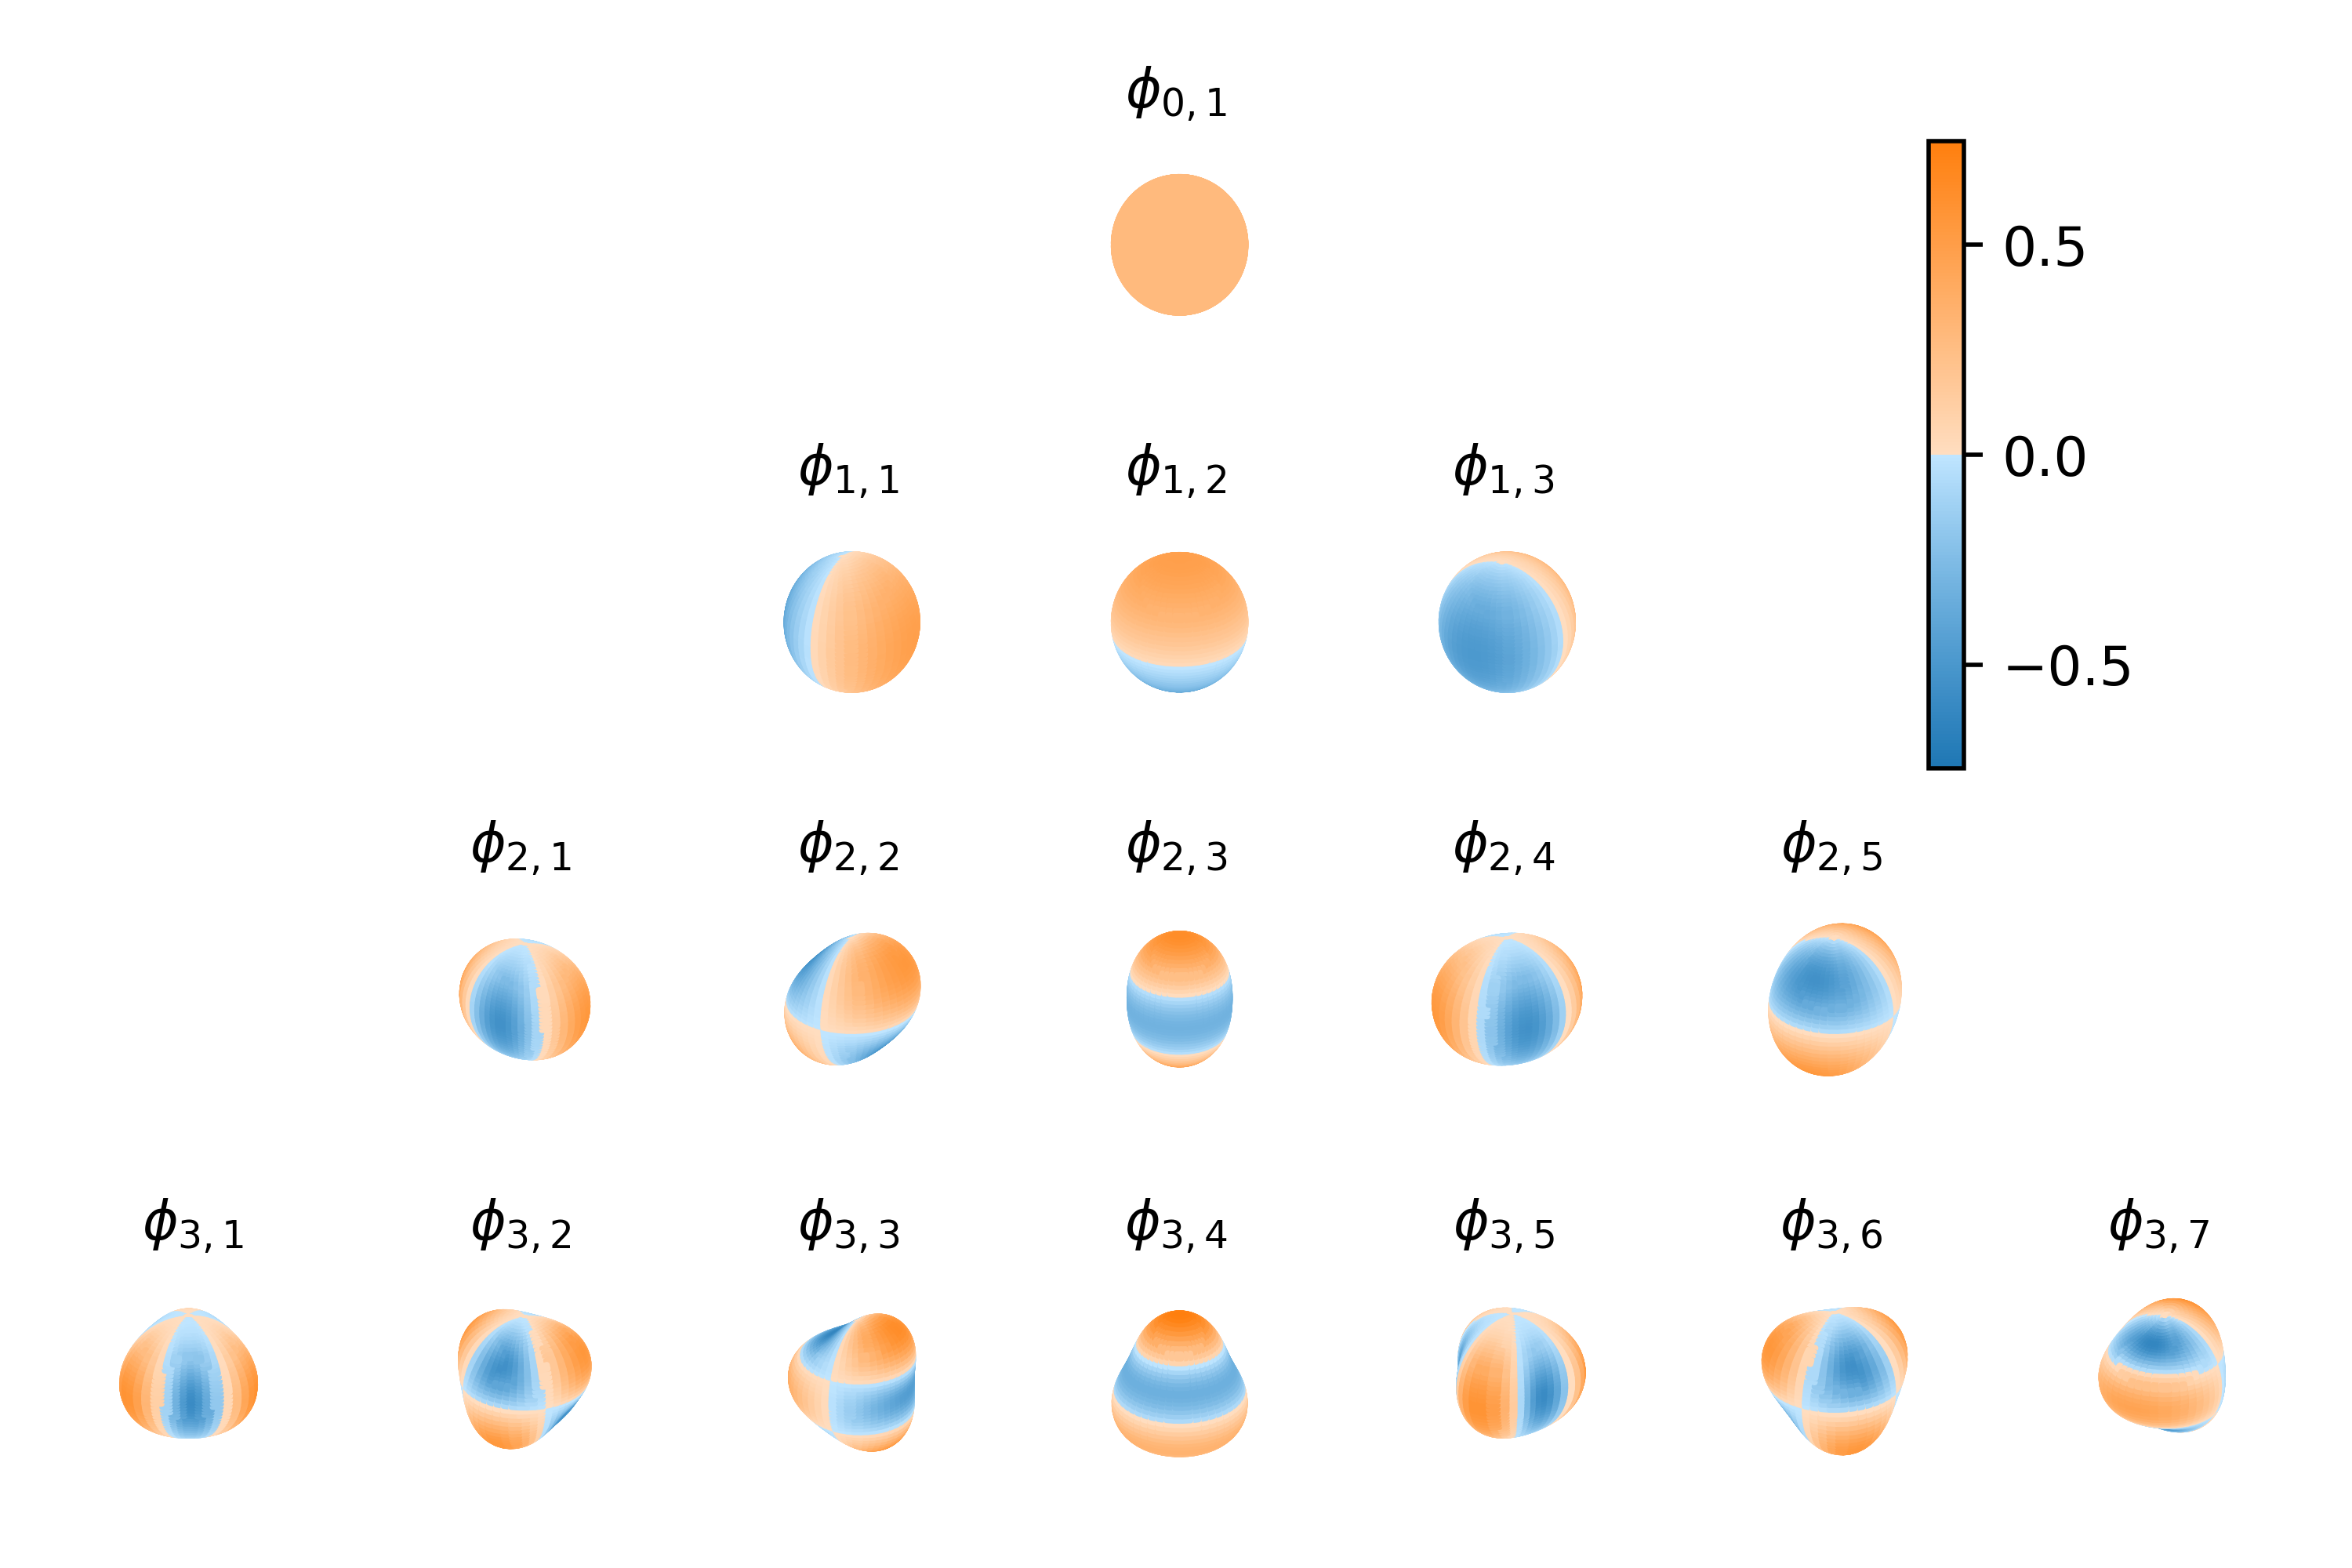
\includegraphics[width=.6\linewidth]{Appendix1/harmonics}
    \caption{Spherical Harmonics}
    \label{fig:appendix:harmonics}
\end{figure}